\section{Flutter}
\ZbSSec{Allgemein}
Bei Flutter handelt es sich um ein Open Source Entwicklungs Kit von Google, welches die Plattform übergreifende App Entwicklung erleichtern soll. Flutter Anwendungen können ohne große Anpassungen unter Windows, Mac OS, Linux, Android und IOS betrieben werden. Die Basis von Flutter ist Dart. Der Aufbau von Flutter unterscheidet sich stark von herkömmlichem objektorientierten Sprachen wie Java oder C\#. Jedes Flutter Projekt besteht aus Widgets und diese enthalten sämtliche Programmlogik.(vgl. \cite{Flutter})

\begin{figure}[h]
\centering
\vspace{0.5cm}

\includegraphics[width=0.8\textwidth]{FLUTTER/images/ZB/flutter_logo.png}
\caption{Flutter Logo \cite{Flutter-Logo}}
\end{figure}

\newpage

\ZbSSec{Architektur}
Die generelle Struktur von Flutter erinnert sehr stark an Android. (vgl. \cite{Flutter-Architektur})

Der Aufbau besteht im Grunde aus 3 Ebenen:
\begin{itemize}
\item \textbf{Embedder}:
Die niedrigste Ebene jeder Flutter App, ist der Embedder, welcher für das Darstellen der Inhalte, mittels nativer Bildschirm Information zuständig ist. Eine weitere Aufgabe ist das Handhaben von Input Events. Die Interaktion mit der Engine Ebene erfolgt über C++ APIs. Ebenfalls im Embedder wird die Dart virtuelle Maschine beherbergt, welche für das Ausführen des Codes auf unterschiedlichen Plattformen zuständig ist. Zusammenfassend ist der Embedder einer der wichtigsten Bestandteile, um Apps flexibel integrieren zu können.

\item \textbf{Engine}:
Die mittlere Ebene einer Flutter App ist die Engine. Die Engine enthält eine große Anzahl von Komponenten, die vor allem für den grundlegenden Betrieb des Frameworks relevant sind. Enthalten sind unter anderem die Grafik-Engine Skia, welche für die optische Darstellung der Flutter App verantwortlich ist.

\item \textbf{Framework}:
Die höchste Ebene einer Flutter ist das Framework. Diese Ebene beinhaltet sämtliche Pakete und Biliotheken, welche für die Entwicklung einer Flutter App notwendig sind. Das Framework ist zum großen Teil in Dart umgesetzt. Die Hauptaufgabe sind Animationen, die Bedienung der App sowie die Erstellung von Widgets.
\end{itemize}
\begin{figure}[h!]
  \centering
  \includesvg[width=0.7\textwidth]{FLUTTER/images/ZB/flutter_architecture.svg}
  \caption{Architektur einer Flutter App \cite{Flutter-Architektur-SVG}}
\end{figure}

\newpage

\ZbSSSec{Vorteile}
Durch die Plattform übergreifende Entwicklung von Flutter, entstehen eine Vielzahl von Vorteilen: (vgl.\cite{Flutter-Vorteile})
\begin{itemize}
\item \textbf{Schnelle Entwicklung}:
Die Entwicklungszeit kann deutlich verkürzt werden, durch die Verwendung derselben Codebasis auf unterschiedlichen Plattformen. Dank der modernen Architektur von Flutter, der hohe Zahl von Komponenten, können Flutter Anwendungen in kürzester Zeit entwickelt werden. Des Weiteren kann auch die Anzahl an Tests drastisch minimiert werden, da auf allen Plattformen dieselben verwendet werden können.

\item \textbf{Einfachere Updates mit Hot Reload}:
Einer der größten Vorteile von Flutter ist die Hot Reload Funktion, welche das Laden von Änderungen am Code innerhalb von Sekunden ermöglicht.

\item \textbf{Hervorragende UI}:
Ein weiterer Vorteil von Flutter ist die Vielzahl an vordefinierten Widgets, welche die Entwicklung um ein Vielfaches beschleunigen, es aber trotzdem ermöglichen, Anwendungen individuell anzupassen.

\item \textbf{Hohe Leistung}:
Die Leistung von Flutter Anwendungen steht der von nativen Anwendungen um nichts nach und ist um ein Vielfaches schneller als die hybride Entwicklung oder andere plattformübergreifende Technologien. Ein weiterer Punkt ist das automatische Umwandeln in nativen Code, somit wird keine mobile SDK als Brücke benötigt.
\end{itemize}

\newpage

\ZbSSSec{Code Beispiel}
Das Code Beispiel zeigt ein simples Hello World in Flutter:

\begin{lstlisting}[style=flutterListingStyle,caption={Hello World - Flutter},label={lst:fluttermain}]
import 'package:flutter/material.dart';

void main() => runApp(HelloWorldApp());

class HelloWorldApp extends StatelessWidget {
  @override
  Widget build(BuildContext context) {
    return MaterialApp(
      title: 'Hello World App',
      home: Scaffold(
        appBar: AppBar(
          title: Text('Hello World App'),
        ),
        body: Center(
          child: Text('Hello World'),
        ),
      ),
    );
  }
}
\end{lstlisting}

\GpSSec{Hot Reload}
Durch die Hot Reload Funktion ist es möglich, Änderungen, die am Code vorgenommen wurden, in Echtzeit darzustellen. Der Hot Reload funktioniert, indem der aktualisierte Code in die laufende Dart VM injiziert wird. Es werden nur die geänderten Teile des Codes neuen kompiliert. Das bedeutet, dass der Zustand von offenen Dialogen oder eingegebenen Daten weiterhin gleich bleibt.
Dadurch muss die Anwendung nicht neu gestartet werden, was einen positiven Effekt auf den Entwicklungsprozess hat, da es dem Entwickler ermöglicht schnell und effektiv Änderungen an der Applikation durchzuführen. (vgl. \cite{Hot-Reload})\\

\GpSSec{Namenskonventionen}
Flutter folgt bestimmten Namenskonventionen, um den Code konsistenter und lesbarer zu machen.(vgl. \cite{name-conventions-desc})

Die wichtigsten Konventionen im Überblick

\begin{itemize}
    \item {\textbf{Camel Case:}} CamelCase wird bei der Benennung von Attributen, Variablen und Methoden verwendet. Hierbei wird das erste Zeichen des Namens kleingeschrieben und jedes Zeichen eines neuen Wortes gro\ss. Beispiel: {\textbf{void generateText(), String office Location}} 
    
    \item {\textbf{Pascal Case:}} Pascal Case wird bei der Benennung von Klassen verwendet. Dabei wird das erste Zeichen eines Namens gro\ss geschrieben. Beispiel: {\textbf{class ThemeHandler}}
    
    \item {\textbf{Snake Case:}} Ist die Konvention, um Dateien zu benennen. Jedes Wort eines Dateinamens wird mit Unterstrichen getrennt und kleingeschrieben.\\ Beispiel: {\textbf{user\_secure\_storage.dart}} 
\end{itemize}

\begin{figure}[h!]
\centering
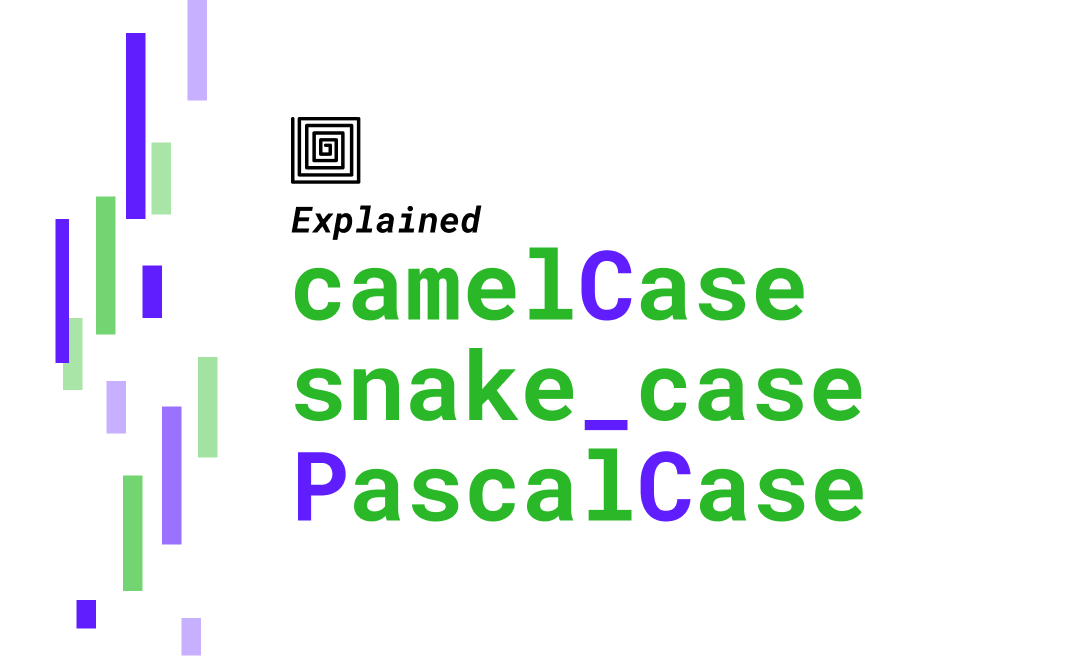
\includegraphics[width=0.6\textwidth]{FLUTTER/images/GP/conventions.png}
\caption{Namenskonventionen\cite{name-conventions}}
\end{figure}

\ZbSSec{Widgets}    
\label{subsec:thero:widgets}
Jede Flutter App besteht zu einem sehr großen Teil aus Widgets. In Widgets werden sämtliche UI-Elemente abgebildet und dargestellt. Das Root Widget, wenn man so will, ist das Scaffold, mit dem beginnt jede Seite in Flutter. Darunter folgt dann eine beliebig lange Folge von Widgets ineinander verschachtelt. Beispiele für Widgets wäre Listen, Buttons, Textfelder und vieles mehr. Des Weiteren gibt es verschiedene Typen von Widgets, Inherited, Stateful und Stateless Widget. Der Unterschied zwischen diesen liegt vor allem darin, wie eine Änderung von Datensätzen realisiert wird. Das heißt, wenn sich Daten von der API ändern, wird die GUI automatisch mit diesen neu geladen.(vgl. \cite{Flutter-Widgets})
\begin{itemize}
    \item \textbf{Inherited Widget}: Wird vor allem für die Übertragung von Parameter an Unterklassen verwendet. Somit muss man nicht jede Variable als Klassen Parameter angeben, sondern schreibt diese einmal in dieses Widget und man kann diese dann aus den Unterklassen aufrufen. Im Abschnitt \ref{inheritedwidget} erfolgt eine genauere Beschreibung anhand eines Beispiels.
    
    \item \textbf{Stateful Widget}: Wird dann verwendet, wenn sich Daten ändern können und somit die UI neu geladen werden muss. Stateful Widgets sind ein wichtiger Bestandteil der Flutter-Anwendungsentwicklung und ermöglichen die Erstellung interaktiver und dynamischer Benutzeroberflächen.

    \item \textbf{Stateless Widget}: Der Unterschied zu den andern beiden Typen liegt darin, dass Stateless Widgets keinen Zustand besitzen und somit im Laufe des Programms nicht verändert werden können. Stateless Widgets sind einfacher zu verwenden und bieten eine gute Performance, da sie einfacher zu berechnen sind.
\end{itemize}

\ZbSSec{Zustands Verwaltung} \label{subsec:thero:statemanagement}
Wenn man als Entwickler das Konzept von Android gewohnt ist und einen Wechsel zu Flutter vollzieht, muss die App-Entwicklung aus einer neuen Perspektive betrachtet werden. Ein großer Unterschied, der zu Android besteht, ist das neu Erstellen, von Widgets, was bei Flutter ``normal`` ist. Wohingegen bei Android, versucht wird, alle Widgets zu modifizieren, damit diese nicht neu gebaut werden müssen. Somit wird Flutter als deklarativ bezeichnet, was so viel bedeute wie, dass immer der aktuelle Stand der Applikation abgebildet wird. (vgl. \cite{Flutter-State-Managment})

\subsubsection{Zustand}
Im Allgemeinen ist ein Zustand alles, was zur Laufzeit der App im Speicher abgelegt wird. Hierbei handelt es sich um  Assets der App, alle Variablen, die das Flutter-Framework über die Benutzeroberfläche speichert, Animationsstatus, Texturen, Schriftarten … Aber wenn man Flutter betrachtet, trifft diese Definition nicht zu. Im Falle von Flutter wäre die Definition eher: Alle Daten, die benötigt werden, um die Benutzeroberfläche zu jedem beliebigen Zeitpunkt neu zu bauen.

\subsubsection{Zustandsänderung}
Wenn der Benutzer einer Flutter Anwendung eine Eingabe auf dem Bildschirm durchführt, z. B. einen Button anklickt, wird die Benutzeroberfläche neu gebaut. Das kann nur dadurch funktionieren, da Flutter auch dafür ausgelegt wurde und die entsprechende Performance mit sich bringt. Dieser Ansatz hat den großen Vorteil, dass es für einen Zustand der Benutzeroberfläche auch nur eine Codebasis geben muss, was wiederum die Komplexität um ein Vielfaches reduziert. Bei Zuständen kann zwischen zwei Arten unterschieden werden.

\subsubsection{Ephemeral state}
Generell ist der ephemere Zustand, jener Zustand, der in einem Widget untergebracht werden soll, z. B.: aktuelle Seite in einer PageView, aktueller Fortschritt einer komplexen Animation. Hierbei handelt es sich vor allem um Widgets, die nur selten benötigt werden, also auch nicht serialisiert werden müssen. Das heißt, dass keine Methoden zur Zustandsänderung benötigt werden. Alles, was in Flutter für Zustände benötigt wird, ist ein Stateful Widget. Wenn eine Seite in einer Anwendung neu geladen werden soll, kann das über setState() durchgeführt werden.

\subsubsection{App state}
Ist das Gegenteil zum ephemeren Zustand. Diese Teile sollen über viele Bereiche der Anwendung verwendet werden z. B. Benutzereinstellungen, Anmeldeinformationen

\subsubsection{Beispiel}
In der nachstehenden Abbildung ist eine Beispielapp zu sehen. Wenn der Benutzer die Option ``Add`` drückt, informiert im Hintergrund das MyListItem das Root Element MyApp (Cart). Dieses kümmert sich dann darum, dass die Seite mit den neuen Daten, neu gebaut wird.

\begin{figure}[h!]
\centering
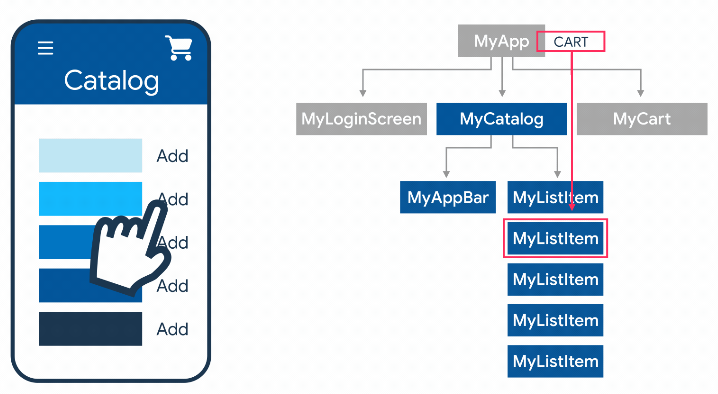
\includegraphics[width=1\textwidth]{FLUTTER/images/ZB/state_example.png}
\caption{Flutter State Beispiel \cite{Flutter-State-Example}}
\end{figure}

\newpage

\subsubsection{Welchen Typ soll man verwenden?}
Die nachfolgende Abbildung zeigt, wann welcher Typ von State verwendet werden soll. Wenn die Daten von vielen oder einigen Widgets benötigt werden, immer App State verwenden. Bei einem einzelnen Widget sollte man den ephemeren Zustand verwenden.

\begin{figure}[h!]
\centering
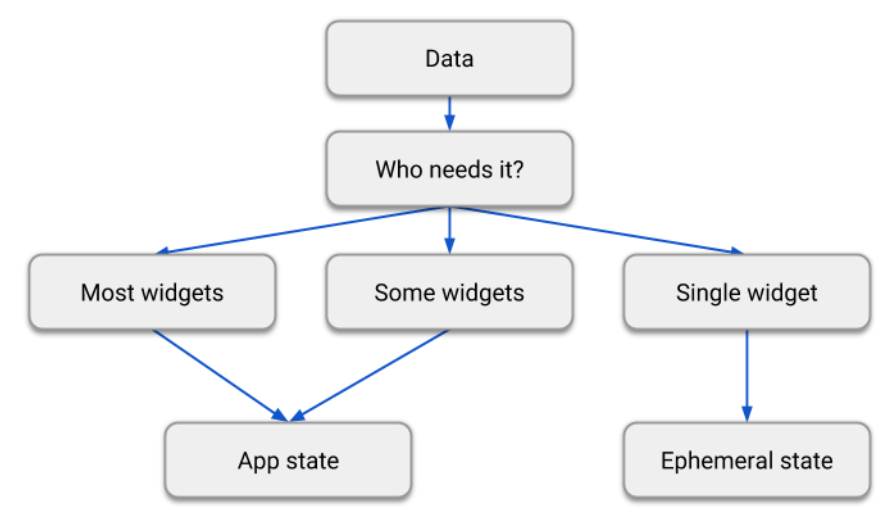
\includegraphics[width=1.0\textwidth]{FLUTTER/images/ZB/which_state.png}
\caption{Flutter State Typ \cite{Flutter-State-Type}}
\end{figure}

\newpage

\subsubsection{Provider}
Provider sind ein sehr wichtiges Konzept in Flutter. Der Aufbau des Providers spiegelt das ``Inversion of Control`` Design Patern wider. Diese werden verwendet, um Zustände und Datenobjekte von einer hierarchisch höheren Ebene, an unterhalb liegende Ebenen zu übergeben. Generell kann der Provider als Vermittler zwischen Widgets und der Datenquelle betrachtet werden. Dadurch kann vermieden werden, dass Widgets direkt auf die Daten an sich zugreifen müssen.(vgl. \cite{Flutter-Provider})

Ein Beispiel zur Implementierung des Provider-Konzeptes erfolgt im Abschnitt\ref{subsec:impl:themehandler}\nameref{subsec:impl:themehandler}
\begin{figure}[h!]
\centering
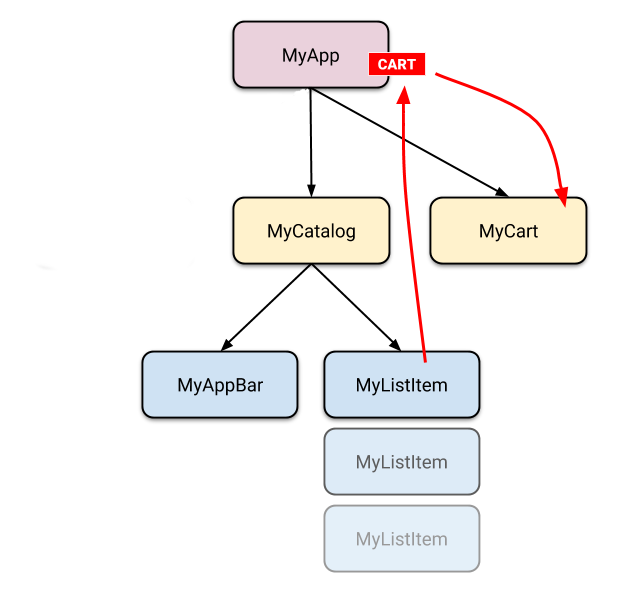
\includegraphics[width=0.9\textwidth]{FLUTTER/images/ZB/provider_example.png}
\caption{Flutter Provider Beispiel \cite{Flutter-Provider-Example}}
\end{figure}






\ZbSSec{Navigator}
Um bei Flutter zwischen Bildschirmen wechseln zu können, gibt es den Navigator. Dieser regelt, dass die Übergänge zwischen den einzelnen Sichten richtig dargestellt werden. Bei der Klasse Navigator besteht die Möglichkeit, Routen direkt in Form der jeweiligen Klasse anzugeben. Was das Problem mit sich bringt, dass es schnell sehr unübersichtlich werden kann. Die weitaus bessere Lösung ist es, eine Routendatei zu verwenden. Diese beinhaltet alle Routen, die es in der App gibt und es wird lediglich der Name der Route bei dem Navigator angegeben. Somit kann die Route im Nachhinein einfach angepasst werden. (vgl. \cite{Navigator})
\\Die Verwendung des Navigators wird im Abschnitt \ref{subsec:impl:routes} \nameref{subsec:impl:routes} beschrieben

\section{Dart}
\ZbSSec{Allgemein}
Die Basis von Flutter ist Dart. Dart stammt ebenfalls von Googele und wurde als Alternative zu JavaScript entwickelt und wird vor allem in der modernen Webentwicklung verwendet. Als großer Unterschied zu JS sollen einige Probleme von JS in Dart behoben worden sein. Dart Code ist an sich bereits im Browser lauffähig und bietet damit die perfekte Basis für Flutter. Durch die Verwendung der DartVM, ist Dart um ein Vielfaches schneller als JS. Dart bietet aber auch die Möglichkeit, außerhalb eines Browsers nativ verwendet zu werden. (vgl.\cite{Dart},\cite{Dart-Aufbau})

\ZbSSSec{Aufbau und Verwendung }
Dart unterstützt wie die meisten Programmiersprachen Variablen, Operatoren, bedingte Anweisungen, Schleifen, Funktionen, Klassen, Objekte und Aufzählungen. Des Weiteren bietet Dart Vererbung und einen objektorientierten Aufbau.

\newpage

\ZbSSSec{Code Beispiel}
Das Code-Beispiel zeigt ein simples 'Hello World' in Dart:
\begin{lstlisting}[style=flutterListingStyle,caption={Hello World - Dart},label={lst:maindart}]
main() {
print('Hello, World!');
}
\end{lstlisting}



\GpSSec{Modifier}\label{subsec:thero:modifier}
In Flutter werden verschiedene Modifier verwendet, um Eigenschaften von Variablen, Funktionen und Widgets zu bestimmen. (vgl. \cite{modifier})


Es erfolgt eine Erklärung der wichtigsten Modifier.

\begin{itemize}
    \item {\textbf{\_private:}} Private Variablen oder Methoden einer Klasse werden mit einem Unterstrich am Anfang ihres Namens bei ihrer Deklaration bestimmt. Private bedeutet, dass die Variablen oder Methoden nur innerhalb einer Klasse sichtbar sind.
    
    \item {\textbf{nullable?:}} Mittels dem Modifier ? kann angedeutet werden, dass eine Methode möglicherweise null zurückgibt oder eine Variable den Wert null annehmen kann. Dieser Modifier wird nach Bekanntgabe des Datentyps angegeben, z. B. {\textbf{int? number}} (Beschreibt, dass der Integer den Wert null annehmen kann)
    
    \item {\textbf{final:}} Eine Variable mit diesem Modifier kann nach ihrer Initialisierung nicht mehr verändert werden.
    
    \item {\textbf{static:}} Methoden oder Variablen einer Klasse können mit diesem Modifier statisch deklariert werden. Dies bedeutet, dass die Variable bzw. Methode einer Klasse nicht zu einer Instanz einer Klasse, sondern zu der Klasse selbst gehört. 
    
    \item {\textbf{const:}} Bedeutet, dass eine Variable nach ihrer Initialisierung nicht mehr verändert werden kann. Der Unterschied zu final ist, dass die Initialisierung bereits bei der Deklaration erfolgen muss.
    
    \item {\textbf{late:}} Deutet auf die spätere Initialisierung einer Variable hin.
    
    \item {\textbf{required:}} Bedeutet, dass ein Parameter einer Funktion  unbedingt notwendig ist.
    
    \item {\textbf{async:}} Deutet auf eine asynchrone Operation hin
    
    \item {\textbf{await:}} Ermöglicht das Warten einer asynchrone Operation, bis der Prozess beendet ist
\end{itemize}





\ZbSSec{Benannte Parameter}
Flutter bietet die Möglichkeit, benannte Parameter zu verwenden. Üblicherweise werden Parameter in Dart-Funktionen über ihre Position übergeben. Dies hat zur Folge, dass der Aufruf einer Methode mit vielen Parameter unlesbarer bzw. unübersichtlicher wird. Genau hier werden benannte Parameter verwendet, um die Lesbarkeit des Codes zu erhöhen.(vgl. \cite{Named-Parameter})
\vspace{0.5cm}
Im nachfolgenden Code Beispiel folgt eine einfache Anwendung eines benannten Parameters. Diese benannten Parameter sind standardmäßig optional, das heißt, dass diese nicht unbedingt übergeben werden müssen. Wenn gewährleistetet sein soll, dass diese Parameter übergeben werden sollen, kann man das Keyword \textbf{required} vor den Datentyp des Parameters schreiben, somit muss dieser Parameter übergeben werden. 

\begin{lstlisting}[caption=Beispiel Methode mit benannten Parameter,label={lst:namedparameter},style=flutterListingStyle]
    final String message;
    final String linenum;
    String? reason;
    //Definition der Methode
    void debugger({required String message, required int lineNum, this.reason}){...}
    //Aufruf aller Paramter
    debugger(message: 'A bug!', lineNum: 44, reason:"Stackoverflow");
    //Aufruf ohne optionalen Paramter
    debugger(message: 'A bug!', lineNum: 44);
    
\end{lstlisting}
Den größten Vorteil, den benannte Parameter mit sich bringen, ist, dass bei dem Methodenaufruf, es um ein Vielfaches leichter ist, die richtigen Parameter zu übergeben. Des Weiteren, ist die Wahrscheinlichkeit um ein Vielfaches geringer, dass die Parameter an der falschen Stelle übergeben werden. 

\GpSSec{Asynchrone Programmierung}  % \label{subsec:thero:async}
Asynchrone Programmierung ermöglicht einem Programm mehrere Prozesse gleichzeitig ablaufen zu lassen, ohne dass die Ausführung der Anwendung blockiert wird. Die Methoden bzw. Funktionen werden so geschrieben, dass eine Abarbeitung der Operationen im Hintergrund erfolgt, ohne dass das Programm auf die Fertigstellung warten muss. (vgl. \cite{asynchrone-programmierung})

\subsubsection{Verwendung von asynchroner Programmierung}
Asynchrone Programmierung wird bei Prozessen benötigt, die mehr Zeit als übliche Operationen benötigen oder die Anwendung blockieren können. 
Die Verwendung der asynchronen Programmierung anhand verschiedener Beispiele
\begin{itemize}
    \item Beim Abruf von Daten aus dem Internet oder eines Servers wird asynchrone Programmierung verwendet, um das Programm während der Abfrage der Daten nicht zu blockieren, dabei wird die Anfrage in einem Hintergrund Thread ausgeführt, um den UI-Thread währenddessen nicht zu blockieren.
    
    \item Ebenfalls wird es bei der komplexen Verarbeitung großer Datenmengen benötigt, um die Anwendung während der Abarbeitung nicht zu blockieren.
    
    \item Die Ausführung von Animationen wird oft in einen asynchronen Prozess ausgelagert, um die Operationen im Hintergrund der Anwendung ablaufen zu lassen, wobei andere Aufgaben im Haupt-Thread schon abgearbeitet werden können.
\end{itemize}

\subsubsection{Future und async}\label{subsec:thero:async}
Mittels dem Modifier {\textit{async}} kann eine Methode in Flutter als asynchron gekennzeichnet werden. Eine mit {\textit{}{async}} gekennzeichnete Funktion ist in der Lage auf die Fertigstellung asynchroner Operationen mit {\textit{await}} zu warten. 
\\
Das {\textit{Future}}-Objekt beschreibt eine Klasse in Flutter, die verwendet wird, um asynchrone Prozesse zu verwalten und zu überwachen. Hierbei stellt das {\textit{Future}} Objekt ein in der Zukunft liegendes Ergebnis oder Wert dar. 
\\
Mittels der Verwendung von {\textit{Future}} und {\textit{async}} ist es möglich, mit {\textit{await}} auf die Fertigstellung des Future Objekts zu warten.

\begin{lstlisting}[caption=Asynchrone Methode zum Abfragen von Daten über einer API,style=flutterListingStyle]
    //Definiton, dass die Methode asynchron ist
    static Future<Response> getReaderCards() async {...}

    //Warten auf Fertigstellung innerhalb einer asynchronen Methoden
    await Data.getReaderCards();
\end{lstlisting}

Anhand dieses Beispiels wird ein typisches Szenario f\"ur die Verwendung asynchroner Programmierung gezeigt. Die Methode {\textit{getReaderCards}} fragt Daten einer API ab, und benötigt daher mehr Zeit als übliche Operationen. Sie gibt aufgrund dessen ein Future Objekt zurück. Der Aufruf der Methode {\textit{await Data.getReaderCards();}} erfolgt nun in einer asynchron gekennzeichneten Methode, um auf die Fertigstellung des Future Objekts zu warten.

\begin{figure}[h!]
\centering
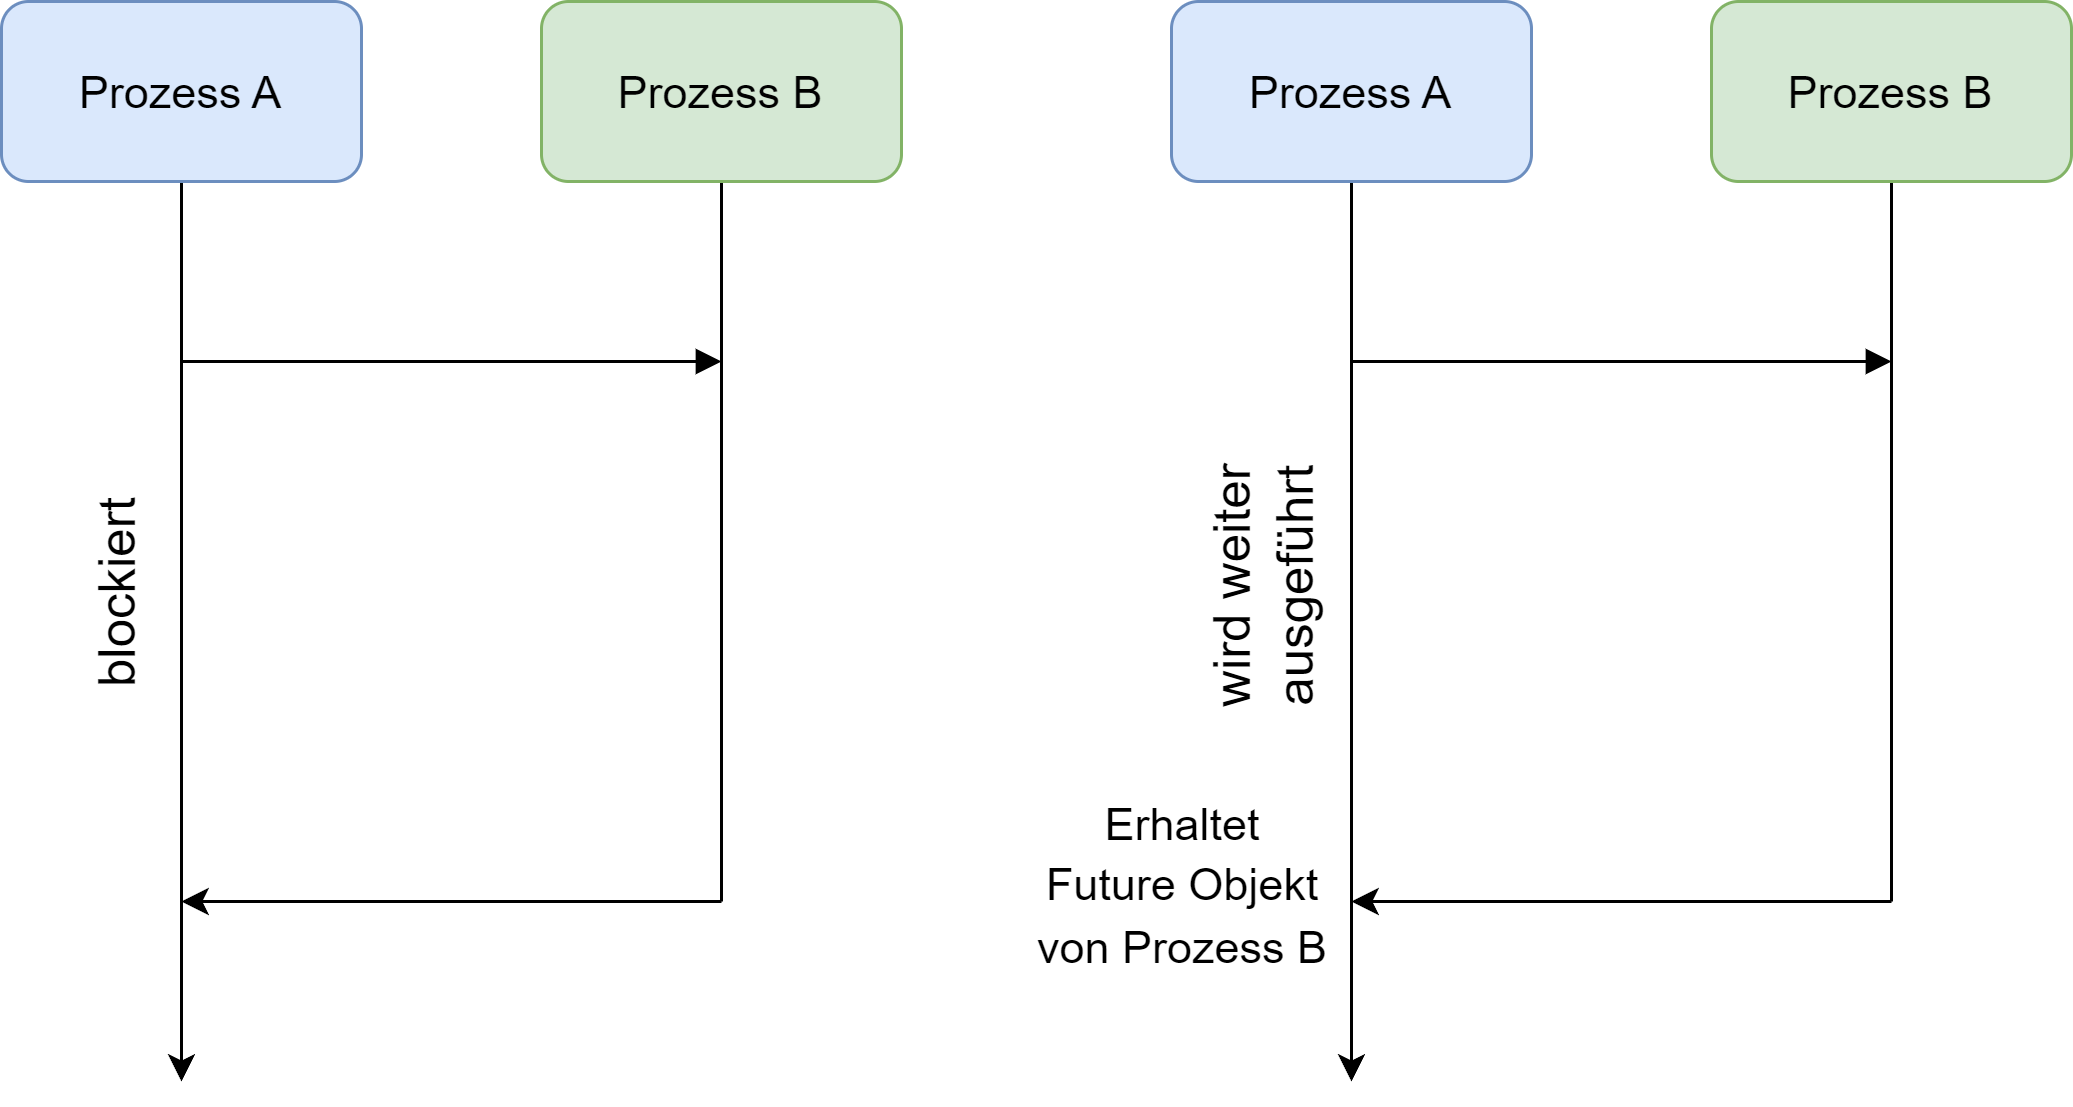
\includegraphics[width=0.6\textwidth]{FLUTTER/images/GP/async.png}
\caption{Unterschied synchronen Operation (links) mit asynchronen (rechts) Operation}
\end{figure}

Als Beispiel wird eine asynchrone Methode im Abschnitt \ref{subsec:impl:apimiddleware} \nameref{subsec:impl:apimiddleware} verwendet und erklärt.

\newpage

\ZbSec{Android - Emulator}
\subsection{Allgemein}
Zum Testen der im Rahmen der Diplomarbeit erstellten Anwendungen werden die Emulatoren von Android Studio genutzt. Android Studio wurde von Google entwickelt. Hierbei handelt es sich um eine freie Entwicklungsumgebung, die basierend auf IntelliJ von JetBrains ist. Das Hauptaugenmerk dieser IDE sind im Rahmen des Projekts die Emulatoren. Um das Ausführen der Flutter Anwendungen, in einer realen Umgebung zu erm\"oglichen. Diese Emulatoren funktionieren fast zu 100 Prozent wie ein reales Endgerät und sind somit ideal zum Testen von Flutter Apps. (vgl.\cite{Android} \cite{Android-AVD})

\subsection{AVD - Android Virtual Device}
Die entwickelten Apps werden nicht direkt im Emulator ausgeführt, sondern auf einem virtuellen Gerät, und zwar auf einem Android Virtual Device. Ein AVD besteht aus einem Hardwareprofile, System Image, Skin und Speicherbereich. Jedes AVD funktioniert wie ein eigenständiges Android-Gerät, also mit eigenem privatem Speicher für Benutzerdaten, installierten Apps und Einstellungen. AVD bietet auch eigene Konfigurations Files, in denen man einstellen kann, was der jeweilige Emulator abbilden soll, ein Tablet, ein Smartphone oder auch andere Geräte. Dadurch kann man seine App auf vielen unterschiedlichen Geräten testen.

\begin{figure}[h!]
  \centering

  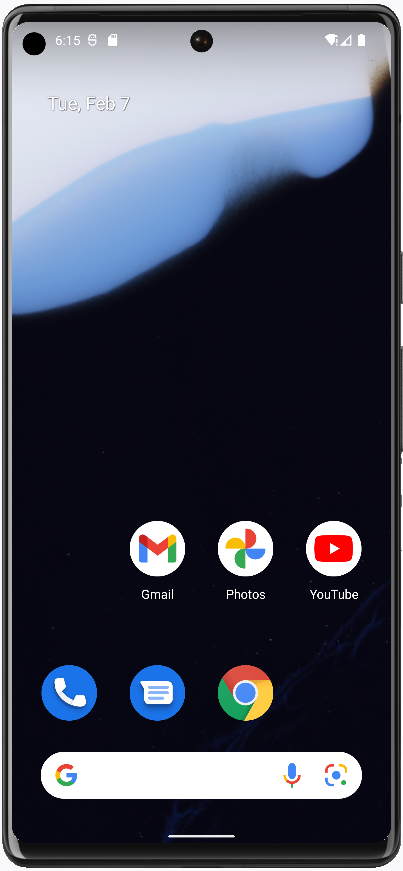
\includegraphics[width=0.15\textwidth]{FLUTTER/images/ZB/android_emulator.png}
  \caption{Android Emulator}
\end{figure}

\newpage

\ZbSec{VSCode}
Als Entwicklungsumgebung wird VSC eingesetzt. VS-Code ist ein freier, quell offener und Plattform übergreifender Code-Editor von Microsoft. Obwohl der Editor  ursprünglich für Webentwickler entwickelt wurde, kann er so gut wie mit allen Sprachen umgehen. Um die gewählte Sprache mit Code Vervollständigung umsetzen zu können, kann man in VS-Code einfach die passenden Extensions installieren. Des Weiteren werden dem Entwickler ein integrierter Debugger, ein Terminal und eine Git Unterstützung geboten. Ein weiteres Merkmal von VS-Code ist, dass es Plattform übergreifend verfügbar ist, was bedeutet, dass er auf Windows, Mac und Linux-Systemen ausgeführt werden kann. (vgl. \cite{VS-Code})

\begin{figure}[h!]
  \centering
  \vspace{1cm}
  
\includegraphics[width=0.20\textwidth]{FLUTTER/images/ZB/vscode_logo.png}
  \caption{Visual Studio Code \cite{VSCode-Logo}}
\end{figure}